\documentclass{ctexart}

\usepackage{pdfpages}

% 超链接
\usepackage{hyperref}
\hypersetup{
    hidelinks,
	colorlinks=true,
	allcolors=black,
	pdfstartview=Fit,
	breaklinks=true
}

\usepackage{listings}
\lstset{
    columns=fixed,       
    numbers=left,                                        % 在左侧显示行号
    numberstyle=\tiny\color{gray},                       % 设定行号格式
    frame=none,                                          % 不显示背景边框
    backgroundcolor=\color[RGB]{245,245,244},            % 设定背景颜色
    keywordstyle=\color[RGB]{40,40,255},                 % 设定关键字颜色
    numberstyle=\footnotesize\color{darkgray},           
    commentstyle=\it\color[RGB]{0,96,96},                % 设置代码注释的格式
    stringstyle=\rmfamily\slshape\color[RGB]{128,0,0},   % 设置字符串格式
    showstringspaces=false,                              % 不显示字符串中的空格
    language=bash,                                       % 设置语言
    basicstyle=\setmainfont{Courier New}
}


% 设置目录显示的深度
\setcounter{tocdepth}{3}

% 设置标号深度
\setcounter{secnumdepth}{3}

% 正文区
\begin{document}

    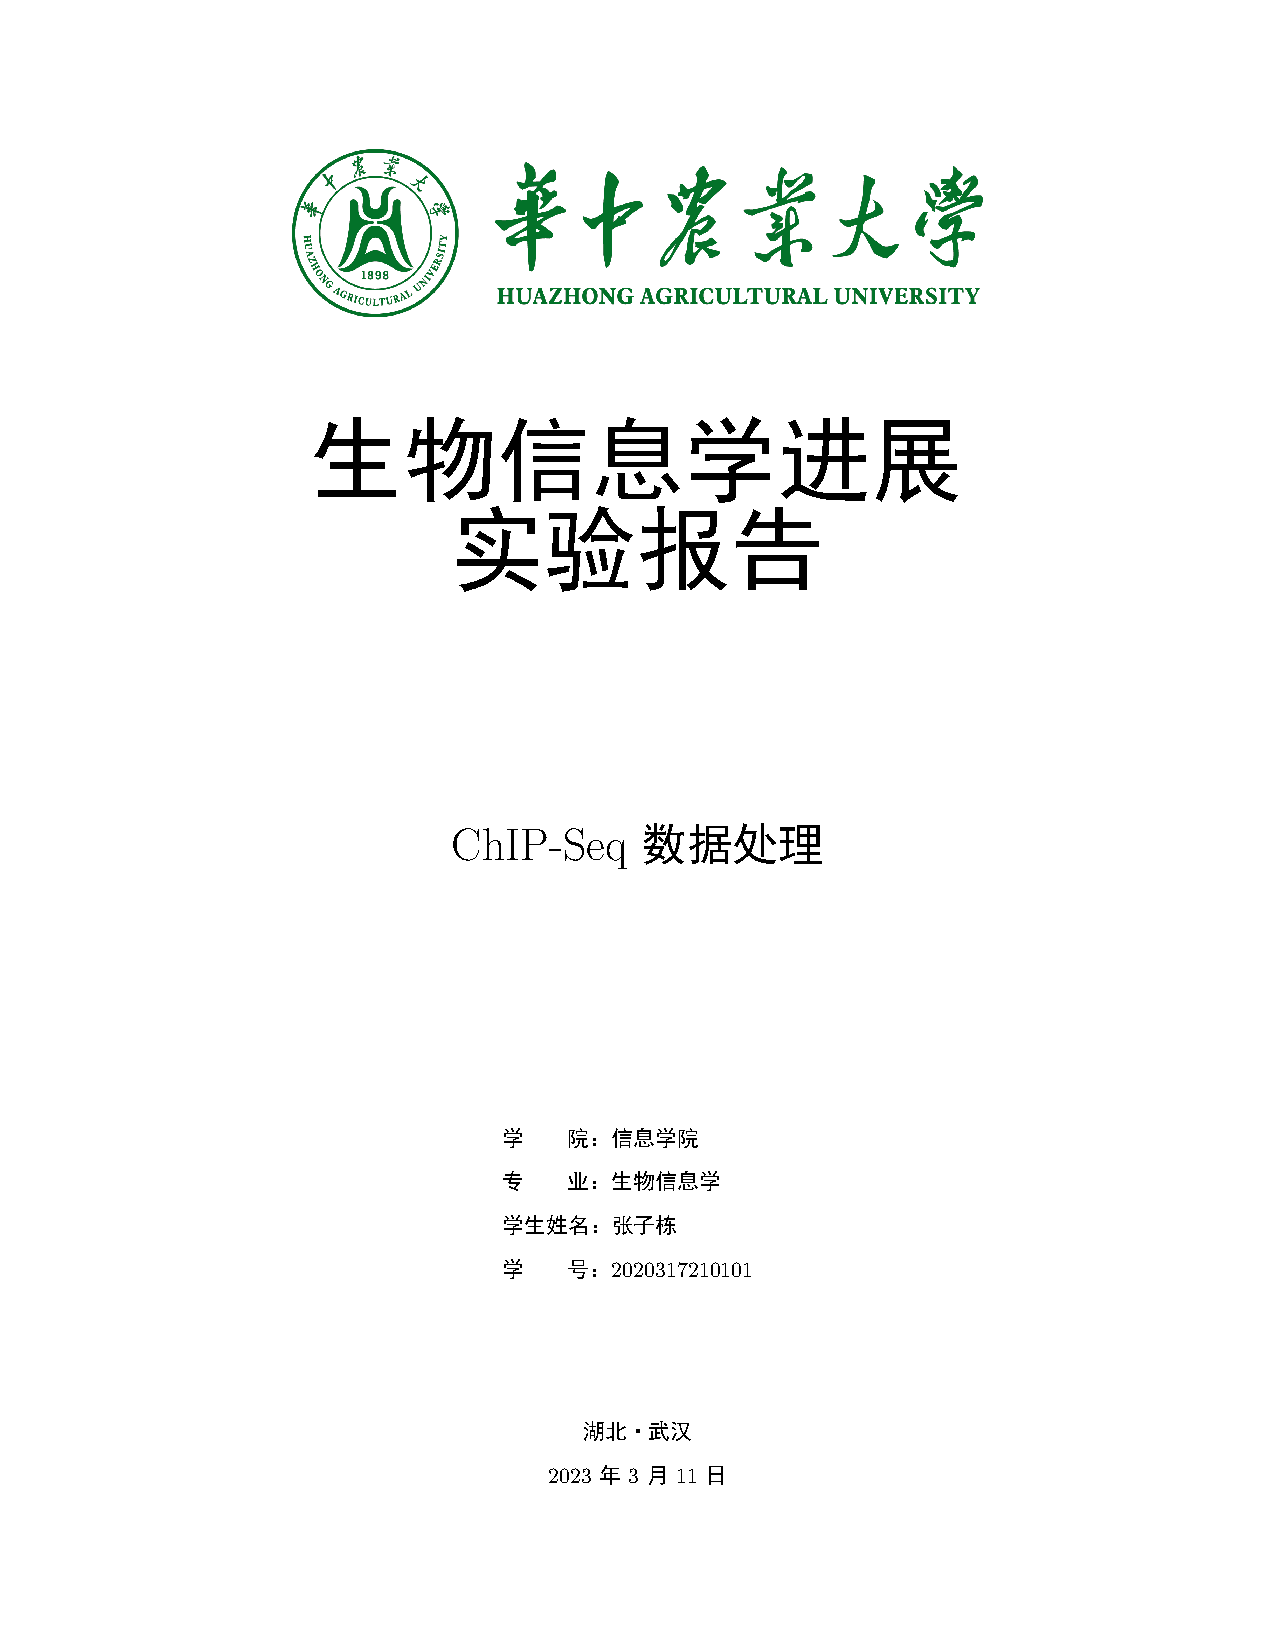
\includepdf[pages={1}]{cover.pdf}

    \clearpage
    \quad
    \thispagestyle{empty}
    \clearpage

    \tableofcontents
    
    % 目录设为页码 0(从正文起为第一页)
    

    % 目录的页脚设为空
    \thispagestyle{empty}

    \clearpage
    \quad
    \thispagestyle{empty}
    \clearpage

    \setcounter{page}{1}

    \section{实验材料}

    \subsection{线虫参考基因组}
    
    \subsubsection{WormBase}

    WormBase 是一个专门收录线虫的基因组信息的数据库,它支持使用线虫作为模式生物的研究者,提供了线虫的基因组序列、注释、变异、表达、互作等数据。WormBase 还包括一个子项目WormBase ParaSite,它收录了其他线虫和扁形动物寄生虫的基因组信息。参考基因组是一个完整的线虫基因序列,基因组注释文件是对参考基因组中的基因、转录本、外显子等特征的描述。

    通过 \href{https://wormbase.org/}{WormBase : Nematode Information Resource}网站获取线虫参考基因组。

    \subsection{线虫 ChIP-Seq 数据}

    来自于上次实验。

    \subsection{实验软件}

    \subsubsection{BWA}

    BWA 是一种能够将差异度较小的序列比对到一个较大的参考基因组上的软件包。它由三个不同的算法组成:BWA-backtrack,BWA-SW 和 BWA-MEM。BWA-backtrack 适用于比对 Illumina 的序列,reads 长度最长能到 100 bp。BWA-SW 和 BWA-MEM 适用于比对长序列,支持的长度
    为 70-1 Mbp;同时支持剪接性比对。

    BWA 的使用需要先对参考基因组建立索引,然后再进行比对。比对的结果是一个 SAM 格式的文件,可以用 samtools 进行后续的处理。

    \begin{itemize}
        \item 建立索引:\verb|index ref.fa|
        \item 比对:\verb|bwa mem ref.fa reads.fq > aln.sam|
        \item 查看帮助:\verb|bwa -h|
    \end{itemize}

    \subsubsection{Bowtie} 

    Bowtie 是一个超快的,存储高效的短序列片段比对程序。它能够将短的 DNA 序列片段(reads)比对到人类基因组或其他较大的参考基因组上。它有两个版本:Bowtie 和 Bowtie2。Bowtie2 是 Bowtie 的升级版,能够比对更长的 reads,支持局部比对和剪接性比对。

    Bowtie 的使用也需要先对参考基因组建立索引,然后再进行比对。比对的结果是一个 SAM 或 BAM 格式的文件,可以用 samtools 进行后续的处理。

    ​	Bowtie 和 BWA 都是常用的短序列比对工具,它们有一些相似之处,也有一些不同之处。

相似之处:

- 都是基于 Burrows-Wheeler Transform(BWT)的算法,利用后缀数组和 FM-index 进行比对。
    - BWT 是 Burrows-Wheeler Transform 的缩写,它是一种数据转换算法,可以把一个文本转换成一个相似的文本,使得相同的字符更容易聚集在一起,从而方便后续的压缩。BWT 的原理是对文本的所有循环移位进行字典序排序,然后取最后一列作为转换后的文本。BWT 是可逆的,也就是说可以从转换后的文本恢复原文本。

- 都能够比对单端或双端的 reads,支持多种格式的输入和输出。

- 都能够处理比对错误和插入缺失,但是对于较长的插入缺失,效果不佳。

不同之处:

- BWA 有两种模式:BWA-MEM 和 BWA-ALN,前者适用于较长的 reads(> 70 bp),后者适用于较短的 reads(< 70 bp)。Bowtie 有两个版本:Bowtie 和 Bowtie2,前者只支持全局比对,后者支持局部比对和剪接性比对。

- BWA 比 Bowtie2 更准确,但是 Bowtie2 比 BWA 更快。BWA 比 Bowtie 更敏感,但是 Bowtie 比 BWA 更节省内存。

- BWA 和 Bowtie2 都能够比对较长的 reads,但是 BWA-MEM 对于较长的 reads 更优于Bowtie2。Bowtie 只能够比对较短的 reads(< 50 bp)。

- BWA 和 Bowtie2 都能够处理比对错误和插入缺失,但是 BWA-MEM 对于较短的插入缺失更优于 Bowtie2。Bowtie 只能够处理比对错误,不能处理插入缺失。

    \section{实验步骤}

    \section{实验结果}

    \section{实验总结}


\end{document}